Диспетчер представляет собой некоторую программу, работающую на процессоре
Microblaze, расположенном на FPGA плате. 
В обязанности диспетчера входят следующие вещи:
\begin{enumerate}
  \item Приём новых задач для выполнения от хоста.
  \item Распределение задач в соответствие с имеющимися ресурсами.
  \item Отслеживание завершения работы задачи и информирование хоста об этом.
\end{enumerate}

Так как Microblaze является программным процессором, диспетчер должен быть,
по возможности, простым и не требующим больших ресурсов.
Для общения с хостом, используется BRAM память, подключённая к Microblaze через
PLB шину. Она невелика по размерам(и разбита на страницы по 4 килобайта),
двухпортовая и синхронная. Одна такая страница отображена в BAR0 PCIe Core,
и через неё происходит обмен сообщениями. Остальная память используется
диспетчер.

В отображённой области памяти статически выделены смещения, по которым будет
происходить запись.
\begin{enumerate}
  \item 0x4 - флаг \texttt {HOST\_DONE}
  \item 0x8 - флаг \texttt {FPGA\_DONE}
  \item 0x14 - адрес для записи результата обработки команды
  \item 0x18 - адрес для записи размера команды
  \item 0х44 - адрес с которого начинается записанная команда.
\end{enumerate}

Для синхронности обмена сообщениями используется следующий протокол, он
представлен на рисунке \ref{mb-sch-auto}. Есть два флага \texttt {HOST\_DONE} и
\texttt {FPGA\_DONE}. Поднятый первый флаг означает, что хост записал своё
сообщение и диспетчер может его обрабатывать. Поднятый второй флаг означает, что
запрос был успешно обработан. Начальное состояние флагов (0,1) задаётся
диспетчером при запуске.
\begin{enumerate}
  \item Состояние флагов (0,1). Хост опускает второй флаг и начинает запись
  сообщения и/или анализ возвращённого значения. По окончании флаги
  устанавливаются в (1, 0)
  \item Состояние флагов (1,0). Диспетчер начинает обработку команды, по
  окончании он записывает результат операции и переводит флаги в (0,1).
\end{enumerate}

\begin{figure}
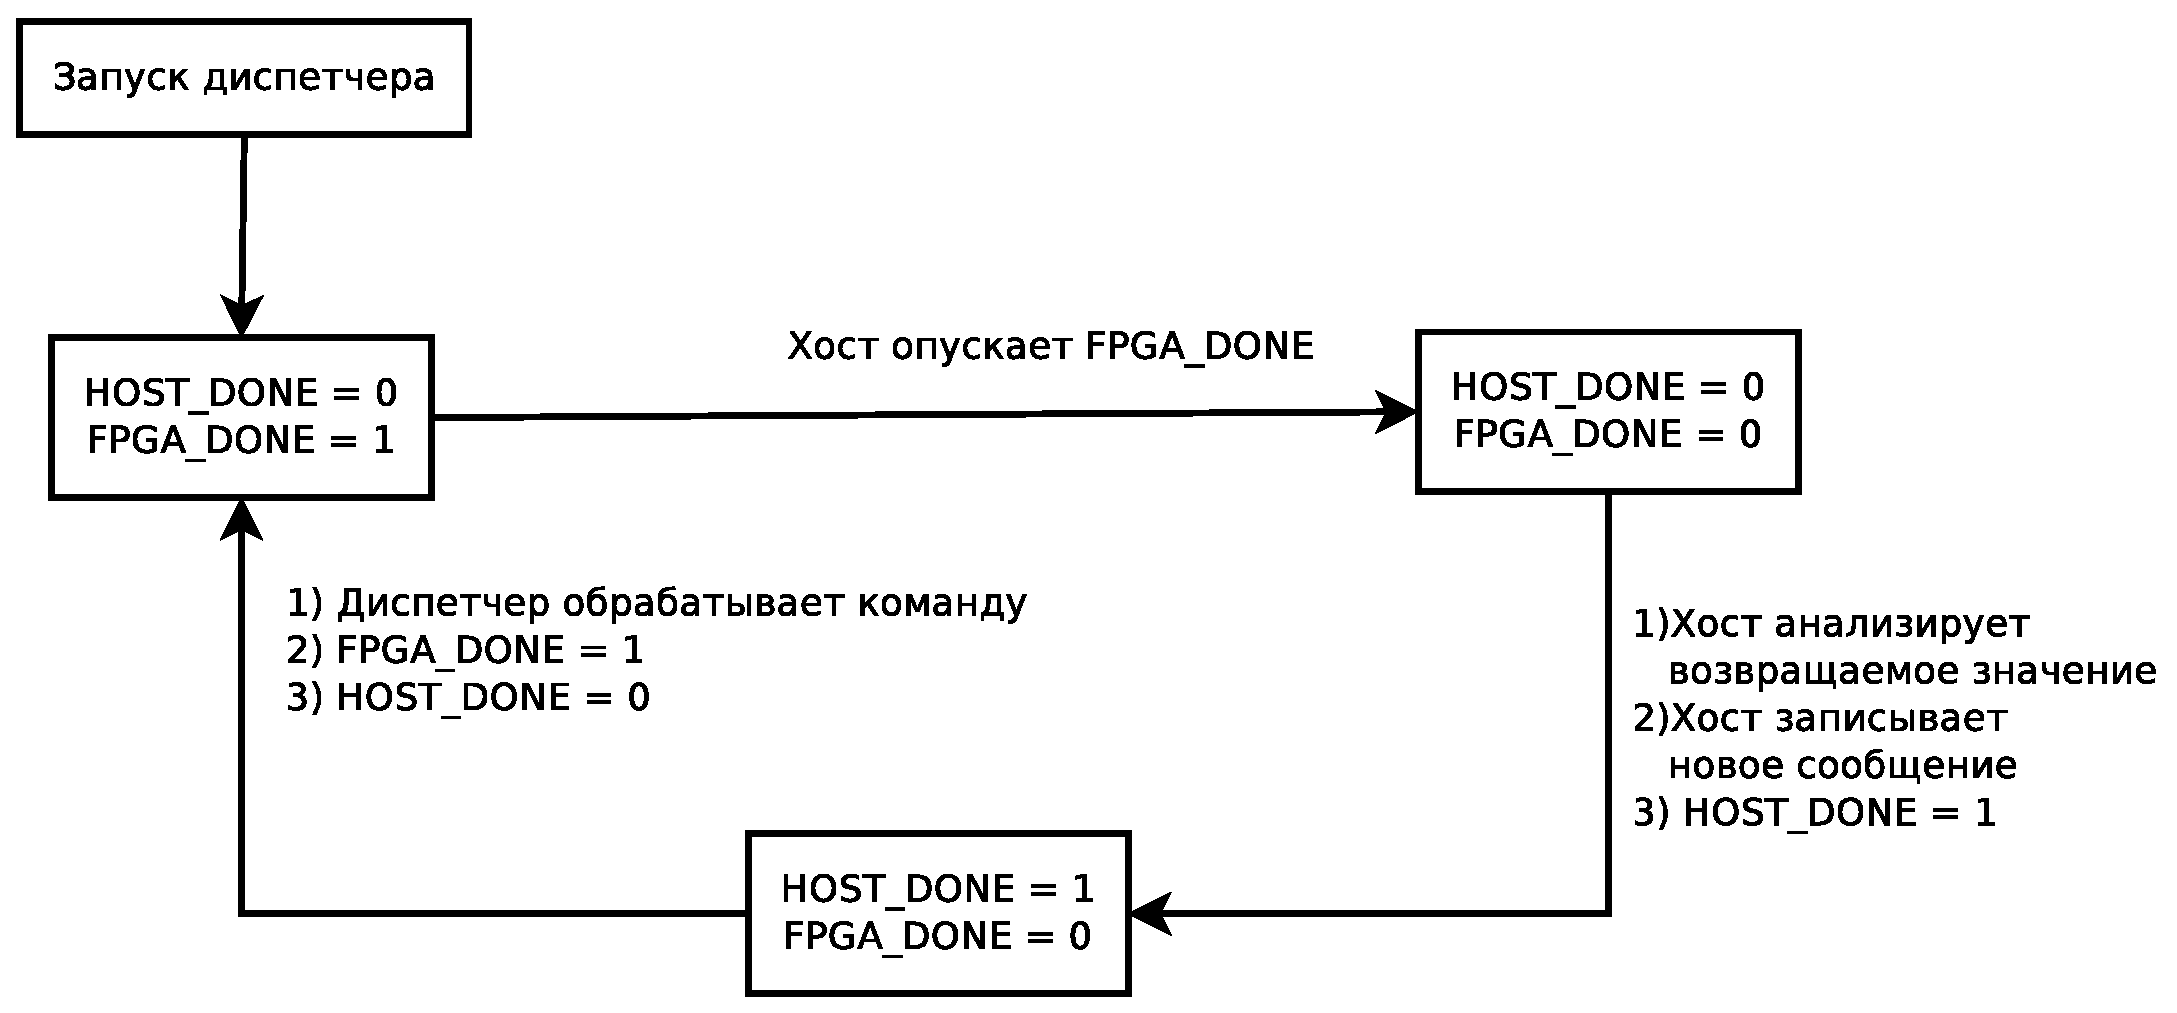
\includegraphics [width=\textwidth]{pictures/mb_sch_auto}
\caption{Протокол обмена сообщениями}
\label{mb-sch-auto}
\end{figure}

Команда имеет следующий формат:\\
<\texttt {kernel\_id} (4 bytes)><\texttt {job\_id} (8 bytes) > \{\texttt{args}\} ~\\

Здесь \texttt {kernel\_id} - уникальный номер ядра, на котором должна
обрабатываться задача, \texttt{job\_id} - уникальный номер задания,
\texttt{args} - аргументы для запуска задачи.

Каждое ядро в системе описывается структурой, хранящей в себе его уникальный
номер, статус(было ли ядру дано какое-либо задание), функция, осуществляющая
запуск задания на нём и функция осуществляющая проверку того, что ядро
закончило работу(например чтение каких-то регистров результата). При
поступление нового задания, обработчик сначала создаёт структуру-обёртку, в
которую, в частности, сохраняются аргументы запуска. Затем в списке ядер ищется
соответствующее заданию ядро и, если оно свободно, задание сразу же
запускается. В противном случае, оно добавляется в очередь заданий для данного
ядра. Таким образом, для добавления в диспетчер поддержки нового ядра,
необходимо написать два обработчика(запуска и проверки результата) и добавить с
структуры данных диспетчера информацию об этом ядре.

В диспетчере постоянно производится опрос ядер на факт завершения выполнения
на них какого-либо задания. Для этого у каждого из имеющихся ядер сначала
проверяется его статус, а затем, если ядру было дано какое-то задание, то
проверяется статус его выполнения. Если какое-то задание завершилось,
в специальный регистр записывается номер задания, а устройство посылает
прерывание, фиксируемое драйвером.  После того, как мы убедимся, что хост считал
номер выполненного задания, при наличии в очереди следующей задачи для этого
ядра, она запускается на нем.

Таким образом всю работу диспетчера можно представить в следующем виде.

  \begin{algo}
\begin{algorithmic}
	\STATE $scheduler\_initialization()$
	\STATE $BRAM\_initialization()$
	\WHILE {\TRUE}
		\STATE $check\_kernels()$
		\IF {$have\_new\_message()$}
			\STATE $process\_message()$
			\STATE $set\_flags()$
		\ENDIF
	\ENDWHILE
\end{algorithmic}
  \caption{Алгоритм работы планировщика}
  \end{algo}
  
Данная реализация справлялась с поставленными задачами, однако по некоторому
размышлению, была предложена новая концепция диспетчера, которая позволяла
перенести его из microblaze в драйвер ядра. Это позволит убрать требование
наличия в целом софтверного процессора на устройстве и избежать активного
ожидания при опросе ядер.
